\documentclass[10pt]{article}
\usepackage[polish]{babel}
\usepackage[utf8]{inputenc}
\usepackage[T1]{fontenc}
\usepackage{amsmath}
\usepackage{amsfonts}
\usepackage{amssymb}
\usepackage[version=4]{mhchem}
\usepackage{stmaryrd}
\usepackage{graphicx}
\usepackage[export]{adjustbox}
\graphicspath{ {./images/} }

\title{LIGA MATEMATYCZNA \\
 LISTOPAD 2009 \\
 GIMNAZJUM }

\author{}
\date{}


\begin{document}
\maketitle
\section*{ZADANIE 1.}
Wykaż, że liczba

\[
2006 \cdot 2008 \cdot 2010 \cdot 2012+16
\]

jest kwadratem liczby naturalnej.

\section*{ZADANIE 2.}
Oblicz pole wielokąta przedstawionego na rysunku wiedząc, że \(0<x<1\).\\
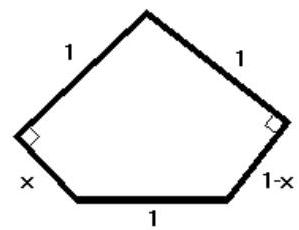
\includegraphics[max width=\textwidth, center]{2024_11_21_08f6750e4347117ff4bbg-1}

\section*{ZADANIE 3.}
Środki kolejnych boków trapezu nierównoramiennego połączono odcinkami. Wykaż, że suma pól powstałych czterech trójkątów jest równa polu otrzymanego czworokąta.

\section*{ZADANIE 4.}
Rozwiąż równanie

\[
1-(2-(3-\ldots-(2009-x) \ldots))=1000
\]

\section*{ZADANIE 5.}
W pięciu skarbonkach była jednakowa ilość monet. Po pewnym czasie okazało się, że wyjęto ze skarbonek połowę wszystkich posiadanych monet. Z pierwszej skarbonki wyjęto 2 monety, z drugiej - 5 monet, z trzeciej - 9, z czwartej - 24 . Nie wiadomo, ile monet wyjęto z piątej skarbonki, ale w każdej skarbonce została co najmniej jedna moneta. Ile było monet na początku i ile monet pozostało w każdej skarbonce?


\end{document}